\section{Environment}

Cryptic crosswords are a popular type of puzzles found in many parts of the 
world. Most commonwealth national newspapers will print cryptic crosswords of 
varying difficulty on a daily basis.

Cryptic crosswords are a unique style of crosswords, in which the answer to 
each given clue is a word puzzle. An answer can only be obtained if the cryptic
clue is read in the correct way. Often when the clue is surface read, the clue 
makes no sense at all. The challenge is to find a way in which the reading of 
the clue leads to a solution.


\section{Problem}

Many users can often become frustrated when a clue appears to be unsolvable. It
is the vast range of possible clues that often makes solving not only 
challenging but interesting as well.

Fundamentally, the overall aim of this project is to develop a piece of 
software that is able to solve any given type of cryptic crossword clue.

By using some form of natural language processing and one or more cryptic 
algorithms, it should be possible to generate an answer to a given clue.

Once a clue has been correctly ``guessed'' it can simply be returned to be 
user. It is the ``guessing'' of the answer that this project will primarily 
focus upon.

\section{Product}


\section{Client}


\section{Users}
The intended customer of the product are users of smartphone and tablets whom are looking to solve all those unsolvable Cryptic Crosswords. The applications will be deployed on the app market for the three listed mobile operating systems which means that the app will be available to anyone who has a compatible device with the required software. The physical deployment of the application is out of the project scope so a price for the deployment will not be discussed.

To determine the users of the product it was decided yo carry out a survey in
order to identify the potential users that actually will be using the product.

The following questions were asked:

\begin{itemize}
    \item Do you play Cryptic Crosswords?
    \item How Often do you play?
    \item Where do you play?
    \item Do you often finish them?
    \item If no to the previous question, what reason don't you finish them?
    \item What is your age group?
    \item When do you play Cryptic Crosswords?
    \item What gender are you?
    \item What is the Highest qualification you have?
    \item What platform is your mobile phone on?
\end{itemize}

The survey was conducted between (date) and (date). It was distributed across
the Department of Computing And Engineering at the University Of Huddersfield,
Facebook and Twitter. The results of this survey are shown in Figure
~\ref{fig:survey_results}


\begin{figure}[H]
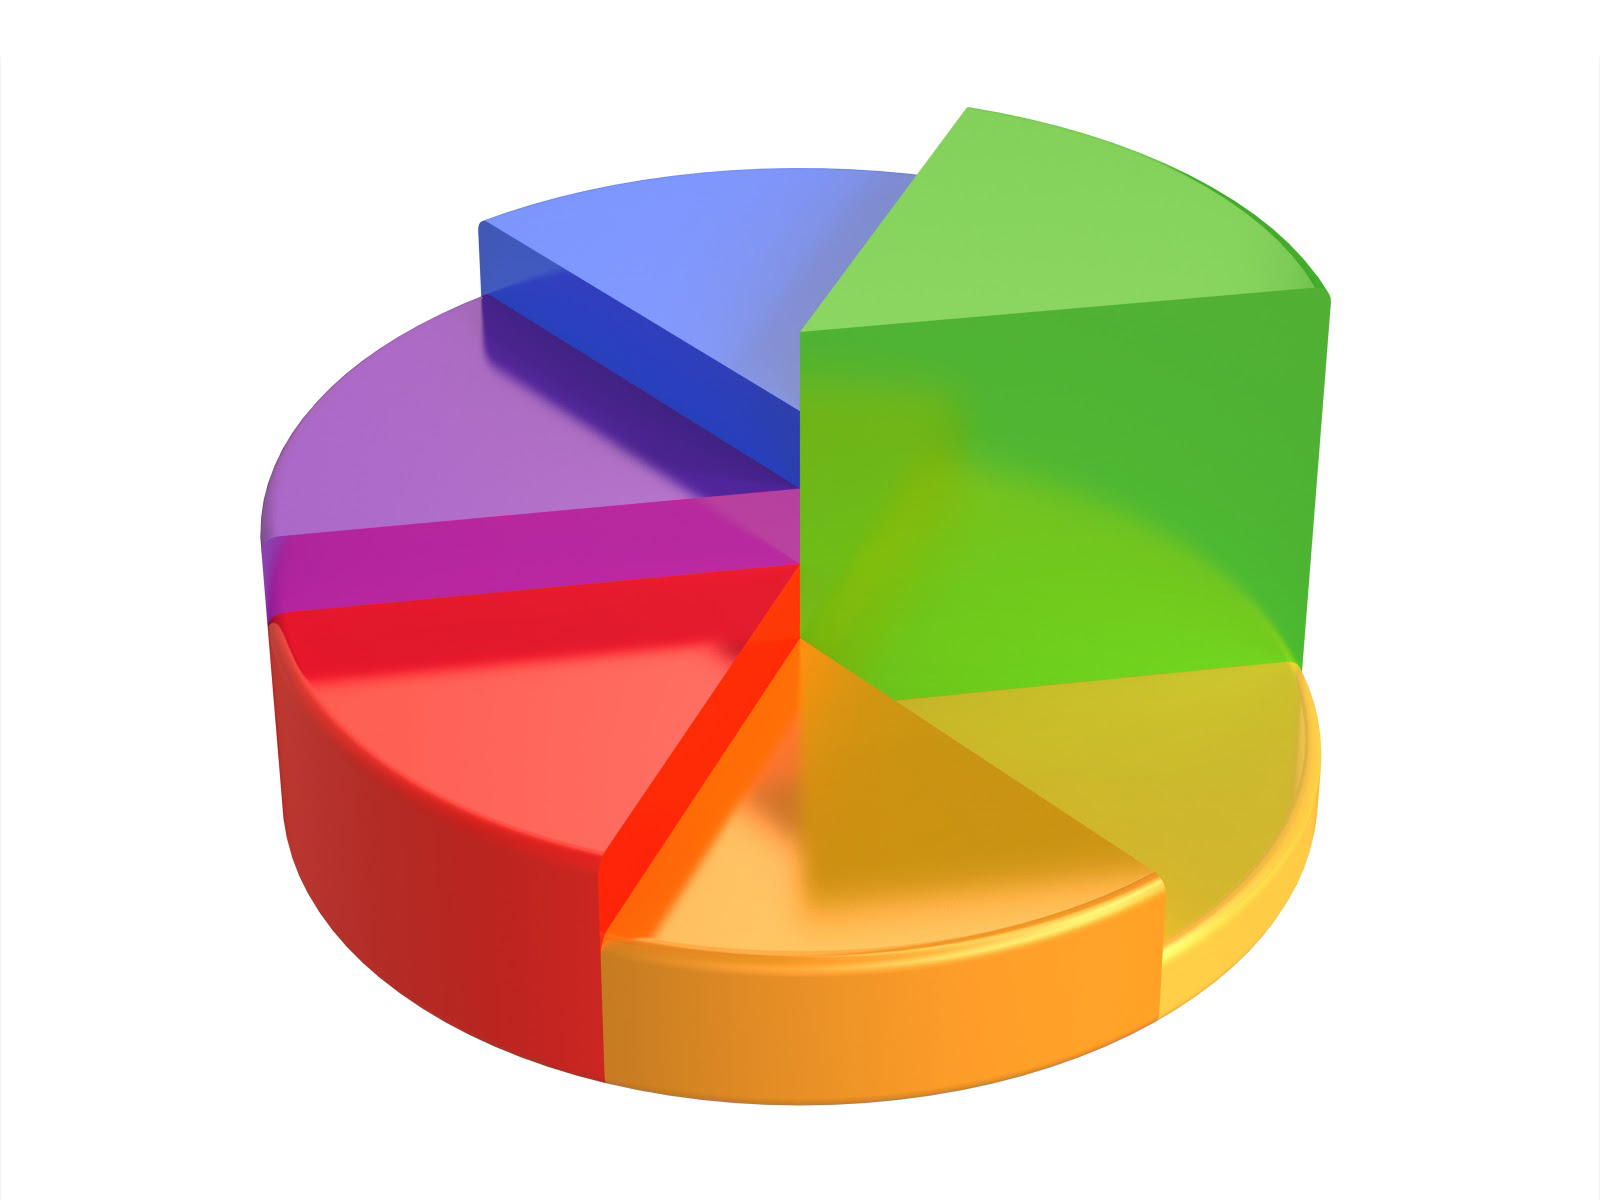
\includegraphics[width=0.9\textwidth]{requirements/project_drivers/survey_results.png}
\caption{Cryptic Crosswords Survey Results}
\label{fig:survey_results}
\end{figure}

From these results it can be deduced that .....